\documentclass{standalone}

\usepackage{tikz}
\begin{document}
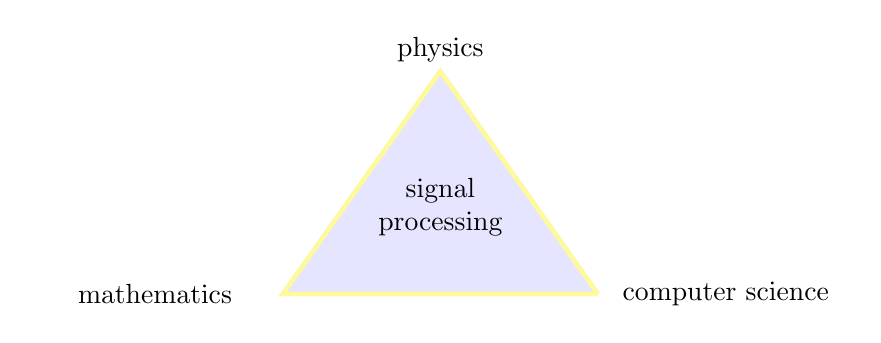
\begin{tikzpicture}
  \node (A) at (2, 0) [right, text width=3cm, align=center]{computer science};
  \node (B) at (-2, 0) [left, text width=3cm, align=center]{mathematics};
  \node (C) at (0, 2.828) [above, ] {physics};


  \filldraw[blue!10, ultra thick] (2, 0) -- (-2, 0) -- (0, 2.828) -- (2, 0);
  \draw[yellow!40, ultra thick] (2, 0) -- (-2, 0) -- (0, 2.828) -- (2, 0);
  \node at (0, 1.1) [text width=5em, align=center]{signal processing};
\end{tikzpicture}
\end{document}
